\documentclass[11pt]{article}

\usepackage[utf8]{inputenc}
\usepackage[T1]{fontenc}
\usepackage{amsmath,amssymb,mathtools}
\usepackage{booktabs}
\usepackage{longtable}
\usepackage[margin=1in]{geometry}
\usepackage{siunitx}
\usepackage{graphicx}
\usepackage[hidelinks]{hyperref}
\usepackage{xcolor}
\usepackage{enumitem}
\usepackage{tikz}
\usetikzlibrary{arrows.meta,positioning,calc,patterns}

\sisetup{per-mode=symbol}

% ---------------------------------------------------------------- macros
\newcommand{\degC}{\ensuremath{^{\circ}\mathrm{C}}}
\newcommand{\Tm}{\ensuremath{T_{m}}}
\newcommand{\Trock}{\ensuremath{T_{r}}}
\newcommand{\Tpcm}{\ensuremath{T_{p}}}
\newcommand{\Rg}{\ensuremath{R_{g}}}
\newcommand{\Rper}{\ensuremath{R_{\mathrm{per}}}}
\newcommand{\Rnear}{\ensuremath{R_{\mathrm{near}}}}
\newcommand{\Rtot}{\ensuremath{R_{\mathrm{tot}}}}
\newcommand{\nft}{\ensuremath{n_{\mathrm{ft}}}}
\newcommand{\Lw}{\ensuremath{L_{w}}}
\newcommand{\rid}{\ensuremath{r_{\mathrm{id}}}}
\newcommand{\Ep}{\ensuremath{E'}}
\newcommand{\md}{\ensuremath{\dot m}}
\newcommand{\qp}{\ensuremath{q'}}
\newcommand{\etast}{\ensuremath{\eta_{\mathrm{st}}}}
\newcommand{\etarte}{\ensuremath{\eta_{\mathrm{RTE}}}}

\title{\textbf{BOREAS: Borehole Array Storage}\\[8pt]
\large A downcomer tube geometry and a conducting formation\\
for latent-heat storage in repurposed wellbores}
\author{J.\ R.\ Barbosa Jr.}
\date{Model version 1.0 \quad\textbullet\quad \today}

\begin{document}
\maketitle

\begin{abstract}
BOREAS replaces two assumptions carried unchanged by the THUMS/P2H2P model
through sixteen versions: the hairpin tube geometry, and the adiabatic
borehole wall (hypothesis H6). The two are not independent, and that is the
central argument of this report. A hairpin requires its melting cascade to be
graded along the \emph{developed tube path} rather than along depth, because
its return leg runs some \SI{45}{\kelvin} below the melting temperature and
would otherwise refreeze material the down leg has just melted. Path grading
places two distinct melting temperatures at the same depth in contiguous
phase-change material, and the conduction between them is \SI{92}{\kilo\watt}
for three hairpins against a duty of order \SI{120}{\kilo\watt} --- a short
circuit across the very cascade the model exists to represent, and a term the
model never contained. Path grading also makes the axial coordinate a path
length rather than a depth, so that each depth is claimed by two tube
segments and no depth-dependent boundary condition can be applied at all.
Replacing the hairpin by $\nft$ downward finned tubes and a single insulated
downcomer removes both obstacles at equal pressure drop and equal storage
volume, and makes the cascade run hot at the bottom, aligning it with the
geothermal gradient rather than opposing it. With the wall conducting, the
storage efficiency ceases to be unity by construction and becomes a
measurement. Field shielding is represented through a depth-dependent well
spacing $B(z)$ appropriate to directionally drilled island fields, where
wellheads sit on \SI{1.83}{\metre} centres and diverge to \SI{70}{\metre} or
more over the storage interval. The formation loss falls from
\SI{75.6}{\percent} of the charge for an isolated well to \SI{12.8}{\percent}
for a thousand-well directional fan and \SI{0.93}{\percent} at island spacing.
\end{abstract}

\tableofcontents
\newpage

\section{Scope and relation to the THUMS series}

\subsection{Why a new series rather than a new version}

P2H2P/THUMS is frozen at v0.16 and remains runnable. Nothing in BOREAS edits
it; the build script hashes the THUMS sources against their recorded stamp and
refuses to proceed if they have moved, so the promise is enforced rather than
asserted. The separation is deliberate. The geometry change is not a refinement
of the hairpin model but a different machine, and the two should be comparable
to one another rather than one silently overwriting the other. In particular,
the \SI{92}{\kilo\watt} parasitic quantified in Section~\ref{sec:hairpin} is a
\emph{result} about the previous geometry, and results require the previous
geometry to remain executable.

\subsection{What is inherited unchanged}

The following are carried over from THUMS v0.16 without modification, and are
documented in the companion model report rather than repeated here:

\begin{itemize}[nosep]
\item the enthalpy formulation (``Formulation C''), in which the stored state
      is $\Ep$, the enthalpy per unit length of tube measured from a
      fully-solid-at-$\Tm$ datum, with the three-branch constitutive curve
      giving subcooled solid, two-phase and superheated liquid;
\item the cyclic steady state (CSS) solver, which marches charge and discharge
      alternately until the end-of-cycle state repeats to tolerance;
\item the quasi-steady melt-layer conduction model and the direction-dependent
      choice of conduction path;
\item the double-stage ORC and the high-temperature heat pump, including
      isentropic machine efficiencies applied inside the cycles;
\item the component-wise exergy audit, the Gouy--Stodola accounting, and the
      treatment of the finite geothermal resource;
\item the single ORC correction pass that resolves the coupling between the
      evaporating temperature and the realised discharge outlet.
\end{itemize}

\subsection{What is new}

Four things, in the order they are developed below: the downcomer tube
geometry (Section~\ref{sec:geometry}); the reinterpretation of the axial
coordinate as a depth, with the cascade orientation that follows
(Section~\ref{sec:coordinate}); the conducting formation
(Section~\ref{sec:formation}); and the depth-dependent field shielding
(Section~\ref{sec:field}).


\section{Nomenclature}

\begin{longtable}{llll}
\toprule
symbol & meaning & unit & default \\
\midrule
\endfirsthead
\toprule
symbol & meaning & unit & default \\
\midrule
\endhead
\multicolumn{4}{l}{\textit{geometry}}\\
$\nft$        & finned tubes per borehole (all downward) & --- & 3 \\
$r_i,\ r_e$   & finned tube inner, outer radius & \si{\metre} & 0.01623,\ 0.02108 \\
$\rid$        & downcomer bore radius & \si{\metre} & 0.02811 \\
$r_{\mathrm{id},o}$ & downcomer outer radius over insulation & \si{\metre} & 0.04096 \\
$r_c$         & equivalent cell radius of one finned tube & \si{\metre} & 0.04555 \\
$R_c$         & casing inner radius, $D_{w}/2$ & \si{\metre} & 0.0889 \\
$r_{co}$      & casing outer radius & \si{\metre} & 0.098 \\
$r_b$         & drilled hole radius & \si{\metre} & 0.110 \\
$\Lw$         & well depth & \si{\metre} & 1524 \\
$L_t$         & developed tube length, $=\Lw$ & \si{\metre} & 1524 \\
$t_{\mathrm{ins}},\ k_{\mathrm{ins}}$ & downcomer insulation thickness, conductivity & \si{\metre},\ \si{\watt\per\metre\per\kelvin} & 0.008,\ 0.007 \\
\midrule
\multicolumn{4}{l}{\textit{formation}}\\
$T_s$         & ground surface temperature & \degC & 18 \\
$\nabla T$    & geothermal gradient & \si{\kelvin\per\kilo\metre} & 45 \\
$k_r,\ \rho c_r$ & formation conductivity, volumetric heat capacity & \si{\watt\per\metre\per\kelvin},\ \si{\joule\per\metre\cubed\per\kelvin} & 2.5,\ \num{2.34e6} \\
$\alpha$      & formation diffusivity, $k_r/\rho c_r$ & \si{\metre\squared\per\second} & \num{1.068e-6} \\
$k_{\mathrm{cem}}$ & annular cement conductivity & \si{\watt\per\metre\per\kelvin} & 1.0 \\
$t_{\mathrm{op}}$ & age of the field at evaluation & \si{yr} & 10 \\
$L_{\mathrm{prod}}$ & depth the geothermal water is produced from & ft & 8000 \\
\midrule
\multicolumn{4}{l}{\textit{field}}\\
$N$           & wells sharing the formation (\texttt{None} $=$ isolated) & --- & --- \\
$B_0$         & wellhead spacing & \si{\metre} & 1.83 \\
$z_{\mathrm{kop}}$ & kickoff depth & \si{\metre} & 300 \\
$\theta$      & effective fan half-angle & \si{\degree} & 45 \\
$R_f(z)$      & cluster radius at depth $z$ & \si{\metre} & --- \\
$B(z)$        & well spacing at depth $z$ & \si{\metre} & --- \\
\midrule
\multicolumn{4}{l}{\textit{thermal}}\\
$\Ep$         & stored enthalpy per unit tube length & \si{\joule\per\metre} & --- \\
$\Tpcm$       & phase-change material temperature & \si{\kelvin} & --- \\
$\Trock$      & undisturbed formation temperature & \si{\kelvin} & --- \\
$K,\ K_\ell$  & tube and formation conductances per unit length & \si{\watt\per\metre\per\kelvin} & --- \\
$\qp$         & heat rate per unit tube length & \si{\watt\per\metre} & --- \\
$\etast$      & storage efficiency, $Q_{\mathrm{dis}}/Q_{\mathrm{ch}}$ & --- & --- \\
$\etarte$     & round-trip efficiency, both parasitics charged & --- & --- \\
$\varepsilon_{\mathrm{cyc}}$ & fraction of the store that cycles & --- & --- \\
\bottomrule
\end{longtable}


\section{Hypotheses}

The THUMS hypotheses H1--H5 are retained. H6 is withdrawn and replaced. The
hypotheses specific to BOREAS are labelled B1--B6.

\begin{description}[leftmargin=2.2em,style=nextline]
\item[B1 --- Parallel downward tubes.] The $\nft$ finned tubes are
hydraulically in parallel, carry equal mass flow, and are thermally identical
at a given depth. Flow in them is downward on charge and upward on discharge.
\item[B2 --- Non-exchanging downcomer.] The downcomer exchanges heat with the
surrounding material only through its insulation, quasi-steadily, and does not
participate in the enthalpy march. Its leak is accounted separately
(Section~\ref{sec:bypass}).
\item[B3 --- One-dimensional formation path.] Heat leaves the borehole
radially. Axial conduction in the formation is neglected, which is justified
by the aspect ratio: the thermal penetration depth over the evaluation horizon
is \SI{46}{\metre} against a well length of \SI{1524}{\metre}.
\item[B4 --- Quasi-steady ground.] Within one charge--discharge cycle the
formation presents a fixed resistance to a fixed far-field temperature. The
cycle time is \SI{10}{\hour} and the formation time constant is years, a
separation of four orders of magnitude.
\item[B5 --- Undisturbed far field.] The reference temperature for the loss is
the \emph{undisturbed} geothermal profile. The warming of the rock immediately
around the field is represented through the time dependence of $\Rg$ and not
as a separate capacitance.
\item[B6 --- Uniform cluster.] All $N$ wells in a field are identical and
equally loaded, so the perimeter loss divides equally among them. Edge wells
in a real cluster lose more than interior ones; this is an averaging, not a
bound.
\end{description}


\section{The hairpin geometry is self-contradictory}
\label{sec:hairpin}

\subsection{What the cascade requires}

The charging water enters the borehole at $\Tm + \Delta T_{4C\text{-}M}$ and
glides $\Delta T_{3C\text{-}2C}$ as it gives up heat, so with the default
values $\Delta T_{4C\text{-}M} = \SI{10}{\kelvin}$ and
$\Delta T_{3C\text{-}2C} = \SI{55}{\kelvin}$ it enters at \SI{160}{\degC} and
leaves at \SI{105}{\degC}. The cascade exists so that the melting temperature
tracks the water: each layer sits a fixed approach below the local fluid
temperature, and the span of melting temperatures matches the glide.

In a hairpin the water traverses two legs in series. Over the second of them
it is already below the top melting temperature --- indeed, with the figures
above, the return leg runs
\begin{equation}
\Tm - (T_{4C} - \Delta T_{3C\text{-}2C}) = 150 - 105 = \SI{45}{\kelvin}
\end{equation}
\emph{below} the melting point. If the cascade were graded by depth, so that
both legs at a given depth saw the same $\Tm$, the return leg would freeze what
the down leg had just melted. The model therefore graded the cascade along the
developed path $z \in [0, 2\Lw]$.

\subsection{What path grading costs}

Path grading is self-consistent, and it is what THUMS did. But it requires two
distinct melting temperatures to coexist at the same depth. With a linear
grade over the path, the difference between the down leg at path position $d$
and the return leg at $2\Lw - d$ is
\begin{equation}
\Delta\Tm(d) = \frac{\text{span}}{2\Lw}\,\big[(2\Lw - d) - d\big]
  = \text{span}\left(1 - \frac{d}{\Lw}\right),
\end{equation}
which is the full span of \SI{48.9}{\kelvin} at the wellhead, falling linearly
to zero at the bottom, with a depth-average of \SI{24.4}{\kelvin}.

These two bodies of material are separated by centimetres of \emph{contiguous}
phase-change material, with no wall between them. Treating the legs as two
parallel cylinders of radius $r_e$ with centre spacing $d_{cc}$ in a medium of
conductivity $k_p$, the conduction shape factor per unit length is
\begin{equation}
\frac{S}{L} = \frac{2\pi}{\operatorname{arcosh}
  \!\left(\dfrac{d_{cc}^{2} - 2r_e^{2}}{2r_e^{2}}\right)},
\qquad
\qp_{\text{leg-leg}} = k_p \frac{S}{L}\, \overline{\Delta\Tm}.
\end{equation}

\begin{table}[h]
\centering
\begin{tabular}{lrrrr}
\toprule
hairpins & legs & $d_{cc}$ & $\qp_{\text{leg-leg}}$ & field total, \% of duty \\
\midrule
1 & 2 & \SI{126}{\milli\metre} & \SI{28}{\watt\per\metre} & \SI{43}{\kilo\watt} \ (\SI{36}{\percent}) \\
2 & 4 & \SI{89}{\milli\metre}  & \SI{41}{\watt\per\metre} & \SI{62}{\kilo\watt} \ (\SI{52}{\percent}) \\
3 & 6 & \SI{73}{\milli\metre}  & \SI{60}{\watt\per\metre} & \SI{92}{\kilo\watt} \ (\SI{77}{\percent}) \\
\bottomrule
\end{tabular}
\caption{Parasitic conduction between the legs of a hairpin, evaluated at the
depth-average temperature difference. This term is absent from the THUMS
model. Note its direction: it \emph{grows} with the number of hairpins, which
the v0.16 parametric study ranked as the single most beneficial design
variable, with an effect of $+\SI{33.7}{\percent}$ on
$\varepsilon_{\mathrm{cyc}}\eta_{\mathrm{RTE}}$.}
\label{tab:shortcircuit}
\end{table}

The heat does not leave the store --- it moves from hot material to cold
material within it --- so this is an exergy destruction and a degradation of
the cascade rather than an energy loss. That does not make it benign. The
cascade is the mechanism by which the store matches a gliding source, and a
parasitic of \SI{77}{\percent} of duty flowing directly down the temperature
grade is a short circuit across the model's central idea.

\subsection{Two further consequences}

\paragraph{Path-graded material is not pourable.} Two melting temperatures at
one depth, in separate radial cells, requires radially segregated cartridges
rather than material placed in layers from the bottom up. This is a
manufacturing requirement that the geometry implies and that was never stated.

\paragraph{No depth-dependent boundary condition is possible.} With
$L_t = 2\Lw$ and $z$ a path length, the map $z \mapsto \text{depth}$ is
two-to-one: each depth is occupied by the down leg at $z = d$ and the return
leg at $z = 2\Lw - d$. A formation temperature that varies with depth would
have two segments claiming it, with no principled way to divide the loss
between them. \emph{This is why the two changes in BOREAS are one change}: the
conducting wall cannot be attached to the hairpin geometry at all.


\section{The downcomer geometry}
\label{sec:geometry}

\subsection{Arrangement}

BOREAS separates the two functions the hairpin conflated. All $\nft$ finned
tubes run downward and exchange heat with the material; a single
\emph{insulated downcomer} returns the whole flow without exchanging. They
meet in a manifold at the bottom of the same borehole.

This is not new construction at depth. A hairpin \emph{is} a bottom
connection --- a U-bend landed at \SI{1500}{\metre} --- and the manifold is
the same class of object: a shop-fabricated assembly run in on the tubing
string, with no cement, no intervention in the formation and no lateral. What
the repurposing inherits is the hole, the casing and the cement, which is
\SIrange{60}{80}{\percent} of a well's cost; everything inside the casing is
new in either geometry.

\begin{figure}[h]
\centering
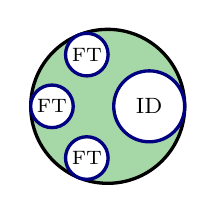
\begin{tikzpicture}[scale=11]
  \fill[green!55!black!35] (0,0) circle (0.0889);
  \draw[very thick] (0,0) circle (0.0889);
  % downcomer, tangent to the wall
  \fill[white] (0.0479,0) circle (0.04096);
  \draw[very thick,blue!50!black] (0.0479,0) circle (0.04096);
  \node at (0.0479,0) {\footnotesize ID};
  % three finned tubes on the opposite side
  \foreach \a in {112,180,248}{
    \fill[white] ({0.0644*cos(\a)},{0.0644*sin(\a)}) circle (0.02458);
    \draw[very thick,blue!50!black] ({0.0644*cos(\a)},{0.0644*sin(\a)})
      circle (0.02458);
    \node at ({0.0644*cos(\a)},{0.0644*sin(\a)}) {\scriptsize FT};}
\end{tikzpicture}
\caption{Borehole cross-section for $\nft = 3$. Shaded: phase-change material,
\SI{60.4}{\percent} of the hole. ID: insulated downcomer,
\SI{82}{\milli\metre} outside diameter, run off-centre. FT: finned tubes over
fins, \SI{49.2}{\milli\metre}. The arrangement is solved rather than sketched;
see Section~\ref{sec:packing}.}
\label{fig:xsec}
\end{figure}

\subsection{Sizing, and why the pressure drop is unchanged}

The downcomer carries the whole flow that the $\nft$ tubes carry between them.
Sizing it for equal velocity therefore means equal total area,
\begin{equation}
\pi\rid^{2} = \nft\,\pi r_i^{2}
\qquad\Longrightarrow\qquad
\rid = r_i\sqrt{\nft}\,,
\label{eq:ridsize}
\end{equation}
giving \SI{28.1}{\milli\metre} for three \SI{1.25}{inch} Sch.\,80 tubes.

The consequence is worth stating carefully, because it is the reason this
geometry was chosen over the alternatives. Let the total well flow be $\md$.
In the hairpin, the flow divides among $n$ hairpins, each a serial path of
area $\pi r_i^2$ and length $2\Lw$, so the velocity is
$u_h = \md/(n\rho\pi r_i^{2})$. In BOREAS, the flow divides among $\nft$ tubes
of the same area over length $\Lw$, and then passes through the downcomer of
area $\nft \pi r_i^2$ over length $\Lw$; by~\eqref{eq:ridsize} the velocity in
both is $u_b = \md/(\nft\rho\pi r_i^{2})$. With $n = \nft$ the velocities are
equal and the total developed length is $2\Lw$ in both cases, so to the extent
that friction factors agree, \emph{the pressure drop is identical}.

This matters because the v0.16 parametric study established that the entire
below-ground influence on round-trip efficiency is pumping: regressing
$\etarte$ on the pumping fraction $f_{\mathrm{pump}}$ alone gives
$R^2 = 0.956$, and within the low-pumping block $\etarte$ varies by less than
one percent. A geometry change that cost pumping would be charged directly
against the only quantity that was moving. The nested-coaxial alternative, in
which the return runs inside each finned tube, preserves storage volume
equally well but divides each bore into two passages plus insulation, leaving
\SI{5.27}{\centi\metre\squared} of each against \SI{19.05}{\centi\metre\squared}
undivided --- a velocity ratio of 1.81 and a pressure-drop factor of 3.3.

\subsection{Packing}
\label{sec:packing}

The downcomer is run off-centre. A concentric arrangement requires
$r_{\mathrm{id},o} + 2(r_e + L_{\mathrm{fin}}) \le R_c$, which for three
\SI{1.25}{inch} tubes in a \SI{7}{inch} hole fails by about
\SI{1}{\milli\metre}. Placing the downcomer tangent to the casing and
distributing the finned tubes on the opposite arc, both tangent circles of
radii $d_{\mathrm{id}} = R_c - r_{\mathrm{id},o}$ and
$d_{\mathrm{ft}} = R_c - (r_e + L_{\mathrm{fin}})$, the smallest angular
offset that clears the downcomer follows from the cosine rule,
\begin{equation}
\cos\theta_{\min} = \frac{d_{\mathrm{id}}^{2} + d_{\mathrm{ft}}^{2}
  - (r_e + L_{\mathrm{fin}} + r_{\mathrm{id},o})^{2}}
  {2\,d_{\mathrm{id}}\,d_{\mathrm{ft}}},
\end{equation}
and the tubes are spread over the remaining $2\pi - 2\theta_{\min}$. This
closes with clearance for $\nft \le 5$; six \SI{1.25}{inch} tubes plus the
downcomer overlap by \SI{12}{\milli\metre} and do not fit. The check is
performed in code and reported beneath the figure, because a schematic that
nobody verifies is a drawing rather than a result.

\subsection{Storage volume and cell radius}

The downcomer occupies cross-section but exchanges no heat with the material
it displaces, so it is subtracted before the cells are formed rather than
counted as a participant:
\begin{equation}
V_{\mathrm{pcm}} = \Lw\Big[\pi R_c^{2}
  - \nft\big(\pi r_e^{2} + n_{\mathrm{fin}} t_{\mathrm{fin}} L_{\mathrm{fin}}\big)
  - \pi r_{\mathrm{id},o}^{2}\Big],
\qquad
\pi r_c^{2} = \frac{\pi\big(R_c^{2} - r_{\mathrm{id},o}^{2}\big)}{\nft}.
\end{equation}
At the default geometry this gives \SI{22.85}{\metre\cubed} of material per
borehole, \SI{60.4}{\percent} of the hole, and $r_c = \SI{45.6}{\milli\metre}$
against a casing radius of \SI{88.9}{\milli\metre}. The cell radius is the
radius at which a tube's melt front meets its neighbour's, and it is not the
borehole wall: a merge limit imposed at the wall would be a factor of two too
permissive and therefore silent at every design point.

\subsection{The downcomer bypass leak}
\label{sec:bypass}

The downcomer is insulated but not adiabatic. Its resistance per unit length
is $R_{\mathrm{ins}} = \ln(r_{\mathrm{id},o}/\rid)/2\pi k_{\mathrm{ins}}
= \SI{8.56}{\metre\kelvin\per\watt}$, two orders above the formation path, so
the two mechanisms do not compete; they are nonetheless reported separately,
because they have different signs and different meanings.

\paragraph{The sign reverses between half-cycles, and the two are not equal.}
On charge the downcomer carries the \SI{160}{\degC} supply \emph{down} past
material grading \SI{101}{\degC} at the top to \SI{150}{\degC} at the bottom,
so heat leaks out of the pipe and into the store. The energy is not lost: it
is deposited in the wrong layer, at a large temperature mismatch. This is an
exergy penalty rather than an energy one, and it is an advantage of this
geometry over the nested coaxial, where the insulated passage carries the
\emph{cold} return and its leak un-stores heat and returns it to the heat
pump. On discharge the downcomer carries the hot outlet back up past the same
material and re-deposits heat just extracted, which is a true capacity loss,
and the larger of the two because the driving difference is larger.


\section{The axial coordinate and the cascade orientation}
\label{sec:coordinate}

\subsection{$z$ becomes a depth}

With the return no longer exchanging, the developed length of a heat-transfer
path is $L_t = \Lw$ rather than $2\Lw$, and the map onto depth is one-to-one.
This single change is what admits a depth-dependent formation.

On charge the water reaches the bottom of the hole through the downcomer
before it has given up any heat, so the finned tubes are entered at the
bottom: the solver coordinate $z = 0$ is the bottom of the well and depth
decreases with $z$,
\begin{equation}
\text{depth}(z) = \Lw - z .
\end{equation}
On discharge the flow reverses --- cold water descends the insulated
downcomer, enters the tubes at the bottom and rises --- so the march is run
with the segment index reversed, and the formation profile is reversed with
it, by exactly the same rule already applied to the melting-temperature
profile. A mirroring error here would place the shielded shallow resistance
against the deep rock, so the orientation is asserted in the parameter
validation rather than left to a comment.

\subsection{The cascade necessarily runs hot at the bottom}

Because the charge water arrives at the bottom undiminished, the hottest
melting layer is at the bottom and the coldest at the top. This is not a free
choice: the geometry determines it.

It is also the favourable orientation. The formation is coldest at the surface
and hottest at depth, so a hot-at-top cascade --- the THUMS arrangement ---
opposes the gradient at both ends. The net driving difference is identical for
either orientation, since the depth-mean of $\Tm(z)$ is unchanged, but the
distribution is not:

\begin{table}[h]
\centering
\begin{tabular}{lrrr}
\toprule
at \SI{8000}{ft}, $\nabla T = \SI{56.5}{\kelvin\per\kilo\metre}$
 & $\Delta T$ at top & $\Delta T$ at bottom & cannot freeze \\
\midrule
hot-at-top (THUMS)     & $+132$\,K & $-55$\,K & \SI{29}{\percent} \\
hot-at-bottom (BOREAS) & $+83$\,K  & $-6$\,K  & \SI{7}{\percent}  \\
\bottomrule
\end{tabular}
\caption{Material held above its melting temperature by the surrounding rock
cannot solidify on discharge, and that capacity is dead --- drilled and paid
for, and unable to cycle. Both orientations have a depth-mean driving
difference of \SI{38.7}{\kelvin}; only the distribution differs.}
\end{table}


\section{The formation}
\label{sec:formation}

\subsection{The series circuit}

Heat leaves the material through four resistances in series, per unit length
of borehole:
\begin{equation}
\Rtot(t) = \underbrace{R_p + R_{\mathrm{cas}} + R_{\mathrm{cem}}}_{\Rnear}
  + \Rg(t),
\end{equation}
with
\begin{align}
R_p &= \frac{\ln(R_c/r_e)}{2\pi\,\nft\,k_p},
&
R_{\mathrm{cas}} &= \frac{\ln(r_{co}/R_c)}{2\pi k_{\mathrm{steel}}},
\\[4pt]
R_{\mathrm{cem}} &= \frac{\ln(r_b/r_{co})}{2\pi k_{\mathrm{cem}}},
&
\Rg(t) &= \frac{1}{2\pi k_r}
  \ln\!\left(\frac{2.5\sqrt{\alpha t}}{r_b}\right).
\label{eq:Rg}
\end{align}

\begin{table}[h]
\centering
\begin{tabular}{lrr}
\toprule
term & value, \si{\metre\kelvin\per\watt} & share \\
\midrule
material to casing, $R_p$      & 0.14543 & \SI{26.5}{\percent} \\
casing steel, $R_{\mathrm{cas}}$ & 0.00034 & \SI{0.1}{\percent} \\
cement, $R_{\mathrm{cem}}$     & 0.01838 & \SI{3.4}{\percent} \\
\textbf{ground}, $\Rg$         & \textbf{0.38413} & \textbf{\SI{70.1}{\percent}} \\
\midrule
total                          & 0.54829 & \\
\bottomrule
\end{tabular}
\caption{The resistance budget at the design point, $t_{\mathrm{op}} =
\SI{10}{yr}$. The casing is thermally invisible and the cement is a rounding
error; the ground resistance is the model.}
\end{table}

Two remarks. First, $R_p$ is the crude term: it treats the $\nft$ tubes as
independent parallel paths to the casing and ignores that those paths crowd
together near the wall. It is a quarter of a total the ground dominates, and
refining it would move the result less than the uncertainty in $k_r$ does ---
across the plausible range $k_r \in [1.5, 3.5]$ the loss varies by a factor of
2.1. Second, $\Rg$ is the only term that depends on time. It grows as the
thermal front spreads, which is why $t_{\mathrm{op}}$ is a parameter of the
case and why a quoted loss figure is meaningless without the age beside it.

\subsection{The undisturbed temperature profile}

\begin{equation}
\Trock(z) = T_s + \nabla T \cdot \text{depth}(z).
\end{equation}
At the default \SI{45}{\kelvin\per\kilo\metre} from \SI{18}{\degC}, the rock
runs from \SI{18}{\degC} at the surface to \SI{86}{\degC} at
\SI{1524}{\metre}. At the central Wilmington value of
\SI{56.5}{\kelvin\per\kilo\metre}, compiled in 1949 from 84 temperature
measurements and the highest known in the Los Angeles basin, it reaches
\SI{104}{\degC} at \SI{5000}{ft} and \SI{156}{\degC} at \SI{8000}{ft} ---
\emph{hotter than the coldest cascade layers}. Those segments gain heat from
the formation. The implementation takes no absolute values anywhere, so a
negative loss is reported as a result rather than absorbed.

\subsection{The gradient and the source temperature are independent}

The wellhead temperature of the geothermal stream is a \emph{lower bound} on
the formation temperature at producing depth: the water cools as it ascends
the production string, and the producing wells may be deeper than the
retrofitted ones. Deriving the gradient from the source temperature writes
that bound as an equality and discards precisely the physics the deficit
represents. Both are therefore specified, and only the inequality
\begin{equation}
T_{\mathrm{source}} \;\le\; T_s + \nabla T\, L_{\mathrm{prod}}
\end{equation}
is enforced --- as a check that can fail, with a warning when the margin falls
below \SI{5}{\kelvin}, which would leave no allowance for the ascent.

\subsection{Coupling to the enthalpy march}

Each segment now has two linear sinks acting on it: the tube at $T_0$ with
conductance $K$, and the formation at $\Trock$ with conductance
$K_\ell = 1/(\Rtot \nft)$, the division by $\nft$ because the per-borehole
conductance is shared among the tubes at that depth. These combine exactly:
for any material temperature $T$,
\begin{equation}
K(T_0 - T) + K_\ell(\Trock - T)
  = (K + K_\ell)\,(T_{\mathrm{eq}} - T),
\qquad
T_{\mathrm{eq}} = \frac{K T_0 + K_\ell \Trock}{K + K_\ell}.
\label{eq:combine}
\end{equation}
The segment advance is therefore called with $(K + K_\ell, T_{\mathrm{eq}})$
and is unchanged in form, remaining implicit in $T$. Adding the loss
explicitly after the step would have been a half-order scheme on a term that
reverses sign with depth.

The split is recovered afterwards without further assumption. If $q_{\Sigma}$
is the net heat the material received over the step, the effective material
temperature follows from $q_{\Sigma} = (K+K_\ell)(T_{\mathrm{eq}} - T_{\rm
eff})$, and then
\begin{equation}
q_{\mathrm{loss}} = K_\ell\,(T_{\mathrm{eff}} - \Trock),
\qquad
\qp_{\mathrm{tube}} = q_{\Sigma} + q_{\mathrm{loss}} .
\label{eq:split}
\end{equation}
Only $\qp_{\mathrm{tube}}$ is charged against the fluid: the formation term is
not the fluid's to pay.

\subsection{What the energy closure becomes}

In THUMS the closure was $|Q_{\mathrm{cum}} - \Delta E|/|Q_{\mathrm{cum}}|$:
everything the tube gave went into storage, because nothing could leave. The
identity is now
\begin{equation}
Q_{\mathrm{tube}} = \Delta E + Q_{\mathrm{loss}},
\end{equation}
and the residual is what remains. This is a bookkeeping identity rather than a
gate --- it cannot fail without an arithmetic error --- but it is retained
because it catches one specific mistake that the split in~\eqref{eq:split}
invites, namely omitting $q_{\mathrm{loss}}$ from the tube duty. It does
\emph{not} catch a sign error, for reasons developed in
Section~\ref{sec:gates}.


\section{Field shielding: $B(z)$}
\label{sec:field}

\subsection{The field is a cone, not an array}

In a directionally drilled island field the wellheads are close and the wells
diverge. THUMS wellheads sit on \SI{6}{ft} (\SI{1.83}{\metre}) centres with
\SI{12}{ft} between double rows, and over 1200 wells reach some 6500 acres
with drift angles to \SI{84}{\degree}. Spacing is therefore a function of
depth, and over the storage interval it varies by more than an order of
magnitude.

The governing quantity is the time for neighbouring thermal fields to merge,
$\tau = B^{2}/\alpha$:

\begin{center}
\begin{tabular}{lr}
\toprule
spacing & merge time \\
\midrule
\SI{1.83}{\metre} (wellhead) & \SI{36}{days} \\
\SI{8}{\metre}               & \SI{1.9}{yr}  \\
\SI{70}{\metre} (base of storage) & \SI{145}{yr} \\
\SI{162}{\metre} (reservoir) & \SI{779}{yr}  \\
\bottomrule
\end{tabular}
\end{center}

The shallow section is a single thermal body within a month; the deep section
is a field of isolated wells. Both occur in the same well.

\paragraph{The two effects oppose one another with depth.} Shallow rock is
cold, so the driving difference is largest exactly where the shielding is
strongest; deep rock is hot, so the driving difference is smallest exactly
where the wells stand alone. This partial cancellation is specific to
directionally drilled island fields and does not arise in purpose-drilled
borehole thermal storage, where the spacing is uniform by design. It is, as
far as we are aware, untreated in the literature, and it is a structural
property of repurposing this particular class of infrastructure.

\subsection{Model}

Above the kickoff point the wells are vertical; below it they fan at an
effective half-angle $\theta$, so with
$R_0 = B_0\sqrt{N/\pi}$,
\begin{equation}
R_f(z) = R_0 + \max\!\big(0,\ \text{depth}(z) - z_{\mathrm{kop}}\big)\tan\theta,
\qquad
B(z) = B_0\,\frac{R_f(z)}{R_0}.
\end{equation}
A real directional programme builds angle over a section and then holds it, so
the fan is not a straight cone; the quantity this feeds is a logarithm, and
the difference is well inside the uncertainty in the spacing data itself.

A shielded well cannot lose what an isolated one would. Once the cells have
merged, the only heat leaving crosses the cluster perimeter, and it divides
among $N$ wells. Taking the semi-infinite-slab flux at that boundary,
$q'' = k_r \Delta T/\sqrt{\pi\alpha t}$, over a perimeter $2\pi R_f(z)$ gives
a loss per well of $q'' \, 2\pi R_f(z)/N$, which written as a resistance is
\begin{equation}
\Rper(z) = \frac{N\sqrt{\pi\alpha t}}{2\pi k_r R_f(z)}\,.
\label{eq:Rper}
\end{equation}
This carries no driving temperature and is therefore a true resistance, so it
enters the series chain directly.

\subsection{Combining the two regimes}

The two are combined by taking the larger resistance:
\begin{equation}
R_{\mathrm{form}}(z) = \Rnear + \max\!\big(\Rg,\ \Rper(z)\big).
\label{eq:maxrule}
\end{equation}
This is not a smooth blend and does not pretend to be. A well cannot lose more
heat than if it stood alone, and a field cannot lose more than its perimeter
admits; whichever constraint binds is the one that governs. The crossover is
sharp in reality as well --- it is the moment the cells merge, and $\tau =
B^2/\alpha$ above shows that moment to be well defined.

\begin{table}[h]
\centering
\begin{tabular}{rrrr}
\toprule
depth, \si{\metre} & $B(z)$, \si{\metre} & $R_{\mathrm{form}}$, \si{\metre\kelvin\per\watt}
 & shielding vs isolated \\
\midrule
0    & 1.8  & 63.62 & $116\times$ \\
300  & 1.8  & 63.62 & $116\times$ \\
600  & 18.6 & 6.39  & $11.7\times$ \\
1000 & 41.1 & 2.99  & $5.5\times$ \\
1524 & 70.4 & 1.81  & $3.3\times$ \\
\bottomrule
\end{tabular}
\caption{$N = 1000$, $\theta = \SI{45}{\degree}$, $t_{\mathrm{op}} =
\SI{10}{yr}$. The shielding weakens by a factor of 35 down the well but never
stops binding: even at the base, where the wells are \SI{70}{\metre} apart,
the field resistance is more than three times the isolated one.}
\end{table}


\section{Verification}
\label{sec:gates}

\subsection{Philosophy}

A check that has never been observed to fail is not evidence. Each gate below
was corrupted deliberately and watched. The two energy checks are reported
together because neither is sufficient alone, and the second exists precisely
because the first proved silent.

\subsection{The adiabatic limit, and an inverted guard}

Driving $k_r \to 0$ must recover hypothesis H6 exactly: zero loss and
$\etast = 1$. On its first execution this test returned $\etast = 0.20$ and a
loss \emph{larger} than the physical case.

The cause was a guard in~\eqref{eq:Rg}. When the argument of the logarithm
falls below unity the line source is outside its validity, and the
implementation returned $\Rg = 0$, intending ``the front has not yet cleared
the hole''. But zero \emph{resistance} is infinite \emph{conductance}: the
expression asserted that the rock was a perfect heat sink, which is the
opposite of what was meant and the most damaging possible failure of that
function. It now returns infinity, and the parameter validation warns rather
than allowing a silent number through. The test passes with zero loss and
$\etast = 1$ to the cyclic convergence tolerance.

\subsection{Why the closure cannot detect a sign error}

Let $q_{\mathrm{loss}}$ be negated in~\eqref{eq:split}. Then
$\qp_{\mathrm{tube}} = q_\Sigma - q_{\mathrm{loss}}$ and the accumulated loss
is $-Q_{\mathrm{loss}}$, so the residual becomes
\begin{equation}
Q_{\mathrm{tube}} - \Delta E - Q_{\mathrm{loss}}^{\,\mathrm{wrong}}
 = \big(\textstyle\sum q_\Sigma - Q_{\mathrm{loss}}\big)
   - \textstyle\sum q_\Sigma - \big(-Q_{\mathrm{loss}}\big) = 0 ,
\end{equation}
identically. The error appears twice with opposite signs and cancels. Measured,
the residual under this corruption is $5\times10^{-15}$ --- machine epsilon.
The closure reads only its own inputs and is therefore blind to the convention
it was written with.

\subsection{A Clausius gate on the loss term}

The independent input the closure lacks is the \emph{state}. Heat must flow
from hot to cold, so $q_{\mathrm{loss}}$ and $(\Tpcm - \Trock)$ must share a
sign at every segment and every step. Accumulating their product,
\begin{equation}
\Sigma \;=\; \sum_{\text{steps}}\sum_{i}
  q_{\mathrm{loss},i}\,\big(T_{p,i} - T_{r,i}\big)\,\Delta z\,\Delta t
  \;=\; \sum K_\ell (\Delta T)^{2} \;\ge\; 0 ,
\end{equation}
which under a reversed convention is $-\sum K_\ell(\Delta T)^2$ and cannot be
positive. The difference from the closure is that $(\Tpcm - \Trock)$ is
evaluated from the marched state rather than from $q_{\mathrm{loss}}$ itself.

\begin{table}[h]
\centering
\begin{tabular}{lrr}
\toprule
corruption & closure & $\Sigma$ \\
\midrule
(none)                           & $2.9\times10^{-16}$ & $+1.64\times10^{11}$ \\
loss omitted from the tube duty  & $5.6\times10^{-1}$ \textbf{fires} & $+1.75\times10^{11}$ silent \\
loss sign reversed               & $5.0\times10^{-15}$ silent & $-3.87\times10^{11}$ \textbf{fires} \\
\bottomrule
\end{tabular}
\caption{Each gate detects exactly what the other cannot. Neither alone would
have been sufficient.}
\end{table}

\subsection{Parameter validation}

Beyond the two energy gates, the case validator checks: the source temperature
against the gradient; the cascade orientation, which must be hot-at-bottom and
whose profile must be in charge-frame indexing; the geometric packing, as a
necessary area condition with a warning when the downcomer must be run
off-centre; the remaining material volume; the fraction of the well whose
melting point lies below the local rock temperature, and so cannot freeze; and
the validity of the line-source form at the requested field age.


\section{Results}

\subsection{Configurations}

\begin{table}[h]
\centering
\begin{tabular}{lrrrrr}
\toprule
configuration & $B$ at base & loss & $\etast$ & $\etarte$
 & $\varepsilon_{\mathrm{cyc}}$ \\
\midrule
isolated well              & ---                & \SI{75.6}{\percent} & 0.244 & 0.072 & 0.452 \\
fan, $N = 100$             & \SI{219}{\metre}   & \SI{54.9}{\percent} & 0.451 & 0.138 & 0.596 \\
fan, $N = 1000$, \SI{70}{\degree} & \SI{190}{\metre} & \SI{28.7}{\percent} & 0.713 & 0.226 & 0.773 \\
\textbf{fan, $N = 1000$, \SI{45}{\degree}} & \SI{70}{\metre} & \textbf{\SI{12.8}{\percent}} & \textbf{0.872} & \textbf{0.281} & \textbf{0.868} \\
array at \SI{1.83}{\metre} & \SI{1.8}{\metre}   & \SI{0.93}{\percent} & 0.991 & 0.323 & 0.931 \\
\bottomrule
\end{tabular}
\caption{All at $t_{\mathrm{op}} = \SI{10}{yr}$,
$\nabla T = \SI{45}{\kelvin\per\kilo\metre}$. The adiabatic value of $\etarte$
is $0.323$.}
\label{tab:results}
\end{table}

Three observations.

\paragraph{The bounding cases differ by two orders of magnitude.} The
isolated-well figure is not a pessimistic estimate of the loss; it is a
different configuration, and one that would not be built. Reporting it alone
would make the concept appear unviable on the strength of an assumption nobody
made deliberately.

\paragraph{The realistic case is material but not fatal.} A thousand wells
fanning at \SI{45}{\degree} lose \SI{12.8}{\percent} of the charge, costing
about \SI{15}{\percent} relative on round-trip efficiency against the adiabatic
value. This is large enough that omitting it would have been a genuine defect
in the model, and small enough that the concept survives it.

\paragraph{The fan angle matters nearly as much as the well count.} Steepening
from \SI{45}{\degree} to \SI{70}{\degree} more than doubles the loss, because
the wells separate faster with depth. In a real field that angle is set by
where the reservoir lies rather than by choice, which makes it a \emph{site}
parameter rather than a design one --- and reframes the question from ``what is
the loss'' to ``over what range of sites does this work''.

\subsection{Insulating the material from the casing}

For an isolated well there is a shallow optimum near \SI{5}{\milli\metre} of
annular insulation, worth some \SI{19}{\percent} in delivered energy before
the volume penalty reverses it; at \SI{20}{\milli\metre} the design is
destroyed outright, since the insulation is removed from the outermost and
largest-area annulus of material. In a field the loss is already below
\SI{1}{\percent}, and insulation trades roughly \SI{11}{\percent} of the
storage volume for nothing.

The sharper observation is that the optimum's \emph{existence} is a symptom
that the isolated-well scope is unphysical. A model whose recommendation is to
insulate is reporting on a configuration that would not be built. Insulation
moves the isolated well from \SI{84}{\percent} lost to \SI{77}{\percent} lost;
spacing moves it to under \SI{1}{\percent}. These are not comparable levers.


\section{Limitations and further work}

\begin{description}[leftmargin=2.2em,style=nextline]
\item[Single field age.] $\Rg$ is evaluated at one $t_{\mathrm{op}}$. The
decay of the loss from the first year to the thirtieth is obtained by repeated
evaluation rather than by an outer loop over years, and the warming of the
rock within the cluster is not represented as a capacitance. At island spacing
that warming is a one-time charge of order \SI{360}{\mega\watt\hour} per well,
roughly 300 daily cycles, after which it is storage rather than loss.
\item[The near-well resistance.] $R_p$ ignores the crowding of the conduction
paths near the casing. It is a quarter of a total the ground dominates.
\item[Uniform cluster.] Hypothesis B6 divides the perimeter loss equally. Edge
wells lose more and interior wells less; representing that requires a
position-resolved field rather than a single $R_f(z)$.
\item[The surface machinery is frozen.] Round-trip efficiency is governed by
the heat-pump lift. Writing the two Carnot factors together,
\begin{equation}
\mathrm{COP}_C \times \eta_C
 = \frac{T_h}{T_h - T_{\mathrm{src}}}\left(1 - \frac{T_0}{T_h}\right)
 = \frac{T_h - T_0}{T_h - T_{\mathrm{src}}},
\end{equation}
which depends on the \emph{lift} and not on how hot the store is --- so
raising $\Tm$ reduces $\etarte$, because the coefficient of performance falls
faster than the power block gains. The lever is the source temperature, and
the same field is considerably hotter at depth than the \SI{60}{\degC}
currently assumed. That is a surface-side study and is not addressed here.
\end{description}


\end{document}
